\documentclass[a4paper, 11pt]{report}
\usepackage{blindtext}
\usepackage[T1]{fontenc}
\usepackage[utf8]{inputenc}
\usepackage{titlesec}
\usepackage{fancyhdr}
\usepackage{geometry}
\usepackage{fix-cm}
\usepackage[hidelinks]{hyperref}
\usepackage{graphicx}
\usepackage{multirow}
\usepackage[english]{babel}

\geometry{ margin=30mm }
\counterwithin{subsection}{section}
\renewcommand\thesection{\arabic{section}.}
\renewcommand\thesubsection{\thesection\arabic{subsection}.}
\usepackage{tocloft}
\renewcommand{\cftchapleader}{\cftdotfill{\cftdotsep}}
\renewcommand{\cftsecleader}{\cftdotfill{\cftdotsep}}
\setlength{\cftsecindent}{2.2em}
\setlength{\cftsubsecindent}{4.2em}
\setlength{\cftsecnumwidth}{2em}
\setlength{\cftsubsecnumwidth}{2.5em}


\begin{document}
\titleformat{\section}
{\normalfont\fontsize{15}{0}\bfseries}{\thesection}{1em}{}
\titlespacing{\section}{0cm}{0.5cm}{0.15cm}
\titleformat{\subsection}
{\normalfont\fontsize{13}{0}\bfseries}{\thesubsection}{0.5em}{}
\titlespacing{\section}{0cm}{0.5cm}{0.15cm}

%=======================================================================================

% #########################
% IMPORTANT - Add student names here!
% e.g. \newcommand{\stud1}{LOWE, David}

\newcommand{\studB}{{FAN, SHING YAM AUSTIN}}
\newcommand{\studC}{{TAN, DAVID CEDRIC CHAN}}

%
% IMPORTANT - Then give your SIDs

\newcommand{\sidB}{{530496287}}
\newcommand{\sidC}{{520657528}}

%
% IMPORTANT - And then update which major each student will focus on

\newcommand{\majB}{{Data Science}}
\newcommand{\majC}{{SW Development}}

% #########################


\pagenumbering{Alph}
\begin{titlepage}
\begin{flushright}

\includegraphics[width=4cm]{USyd}\\[1cm]
\end{flushright}

\begin{centering}
\textbf{\huge INFO1111: Computing 1A Professionalism}\\[0.75cm]
\textbf{\huge 2024 Semester 1}\\[2cm]
\textbf{\huge Skills: Team Project Report}\\[2cm]

\textbf{\large Submission number: ?? Add your details}\\[0.5cm]
\textbf{\large Github link: ?? Add your details}\\[0.75cm]
\textbf{\huge Team Members:}\\[0.75cm]

\begin{tabular}{|p{0.25\textwidth}|p{0.13\textwidth}|p{0.12\textwidth}|p{0.12\textwidth}|p{0.22\textwidth}|}
	\hline
	\multirow{2}{*}{Name} & \multirow{2}{*}{Student ID} & Target * & Target * & \multirow{2}{*}{Selected Major} \\
	 & & Foundation & Advanced & \\
	\hline
	\hline
	\raggedright{\studB} & \sidB & A & NA & \majB \\
	\hline
	\raggedright{\studC} & \sidC & A & NA & \majC \\
	\hline
\end{tabular}
\\[0.5cm]
\end{centering}

* Use the following codes:
\begin{itemize}
\setlength\itemsep{0em}
\item NA = Not attempting in this submission
\item A = Attempting (not previously attempting)
\item AW = Attempting (achieved weak in a previous submission) 
\item AG = Attempting (achieved good in a previous submission)
\item S = Already achieved strong in a previous submission
\end{itemize}

\thispagestyle{empty}
\end{titlepage}
\pagenumbering{arabic}


%=======================================================================================

\tableofcontents

%=======================================================================================

\newpage
%=======================================================================================

\newpage
\section{Task 1 (Foundation): Core Skills}

% =======================================================
\newpage
\subsection{Skills for \majB: \studB}
Data Analysis (DTAN):
\\[1em]
Data Analysis is a foundational skill of data science. it is the skill to encompassing the processes of examining, cleansing, transforming, and modeling data to uncover insights and support decision-making \cite{Dtan1}.
\\[1em]
This skill enables data scientists to identify patterns, trends, and correlations within large and complex datasets. It helps draw meaningful insights to improve business operations, customer behavior, markets trends, and many more \cite{Dtan3}. 
\\[1em]
Data scientists leverage data analysis to optimize operations, predict future outcomes, manage risks, and deliver personalized experiences in numerous domains and industries. A good data scientist can extract actionable insights from data by understanding statistical methods, data manipulation techniques, domain-specific knowledge. They also translate raw data into meaningful information that helps organizations make data-driven decisions optimize processes and stay ahead of the curve in today’s marketplace \cite{Dtan2}\cite{Dtan3}.
\\[1em]
\\[1em]
\noindent Machine Learning (MLHE):
\\[1em]
Machine Learning is another critical skill of data science. In the digital age, organizations generate vast quantities of data from huge sources such as social media, sensors, IoT devices, and more. Machine learning can be defined as algorithms that learn from data and make predictions or decisions without being explicitly programmed \cite{Mlhe1}.
\\[1em]
Mastering MLHE allow data scientists to handle with complex & big data, and automation of tasks via, e.g., by using it, handling complex & big data, and automation of tasks: machine learning techniques can automatically identify patterns, trends, and correlations that might not be immediately obvious through manual analysis, and Machine learning also automates Data preprocessing, Feature Engineering, and Model Selection enable data scientists to focus on strategic, creative work. This increases productivity and growth of data-driven solutions \cite{Mlhe2}. 
\\[1em]
\\[1em]
\noindent Data Visualization (DATA):
\\[1em]
Data Visualization is an important skill in the field of data science it supports and improve data exploration, and communication, and collaboration. This skill enables data scientists to better understand complex datasets by coordinating visual representations , such as charts, graphs and dashboards. It therefore help to translate raw data into human-friendly formats where we can draw patterns, trends, and outliers among data \cite{Data1}\cite{Data2}.
\\[1em]
Additionally, DATA help in designing visual representations and information that enhances presentations. It “makes-up” the real Visualization but including visual elements with contextual information and analysis to create a sensible story for non-experts. For this reason, data visualization helps vital in ensures better decision making amongst Organization teams including Administration \cite{Data1}.
\\[1em]
\\[1em]
Screenshot for command entered and output of compiling from the command line & uploading commit to local repository: (each figure includes the output from the previous command entered)
\begin{figure*}[H]
    \centering
    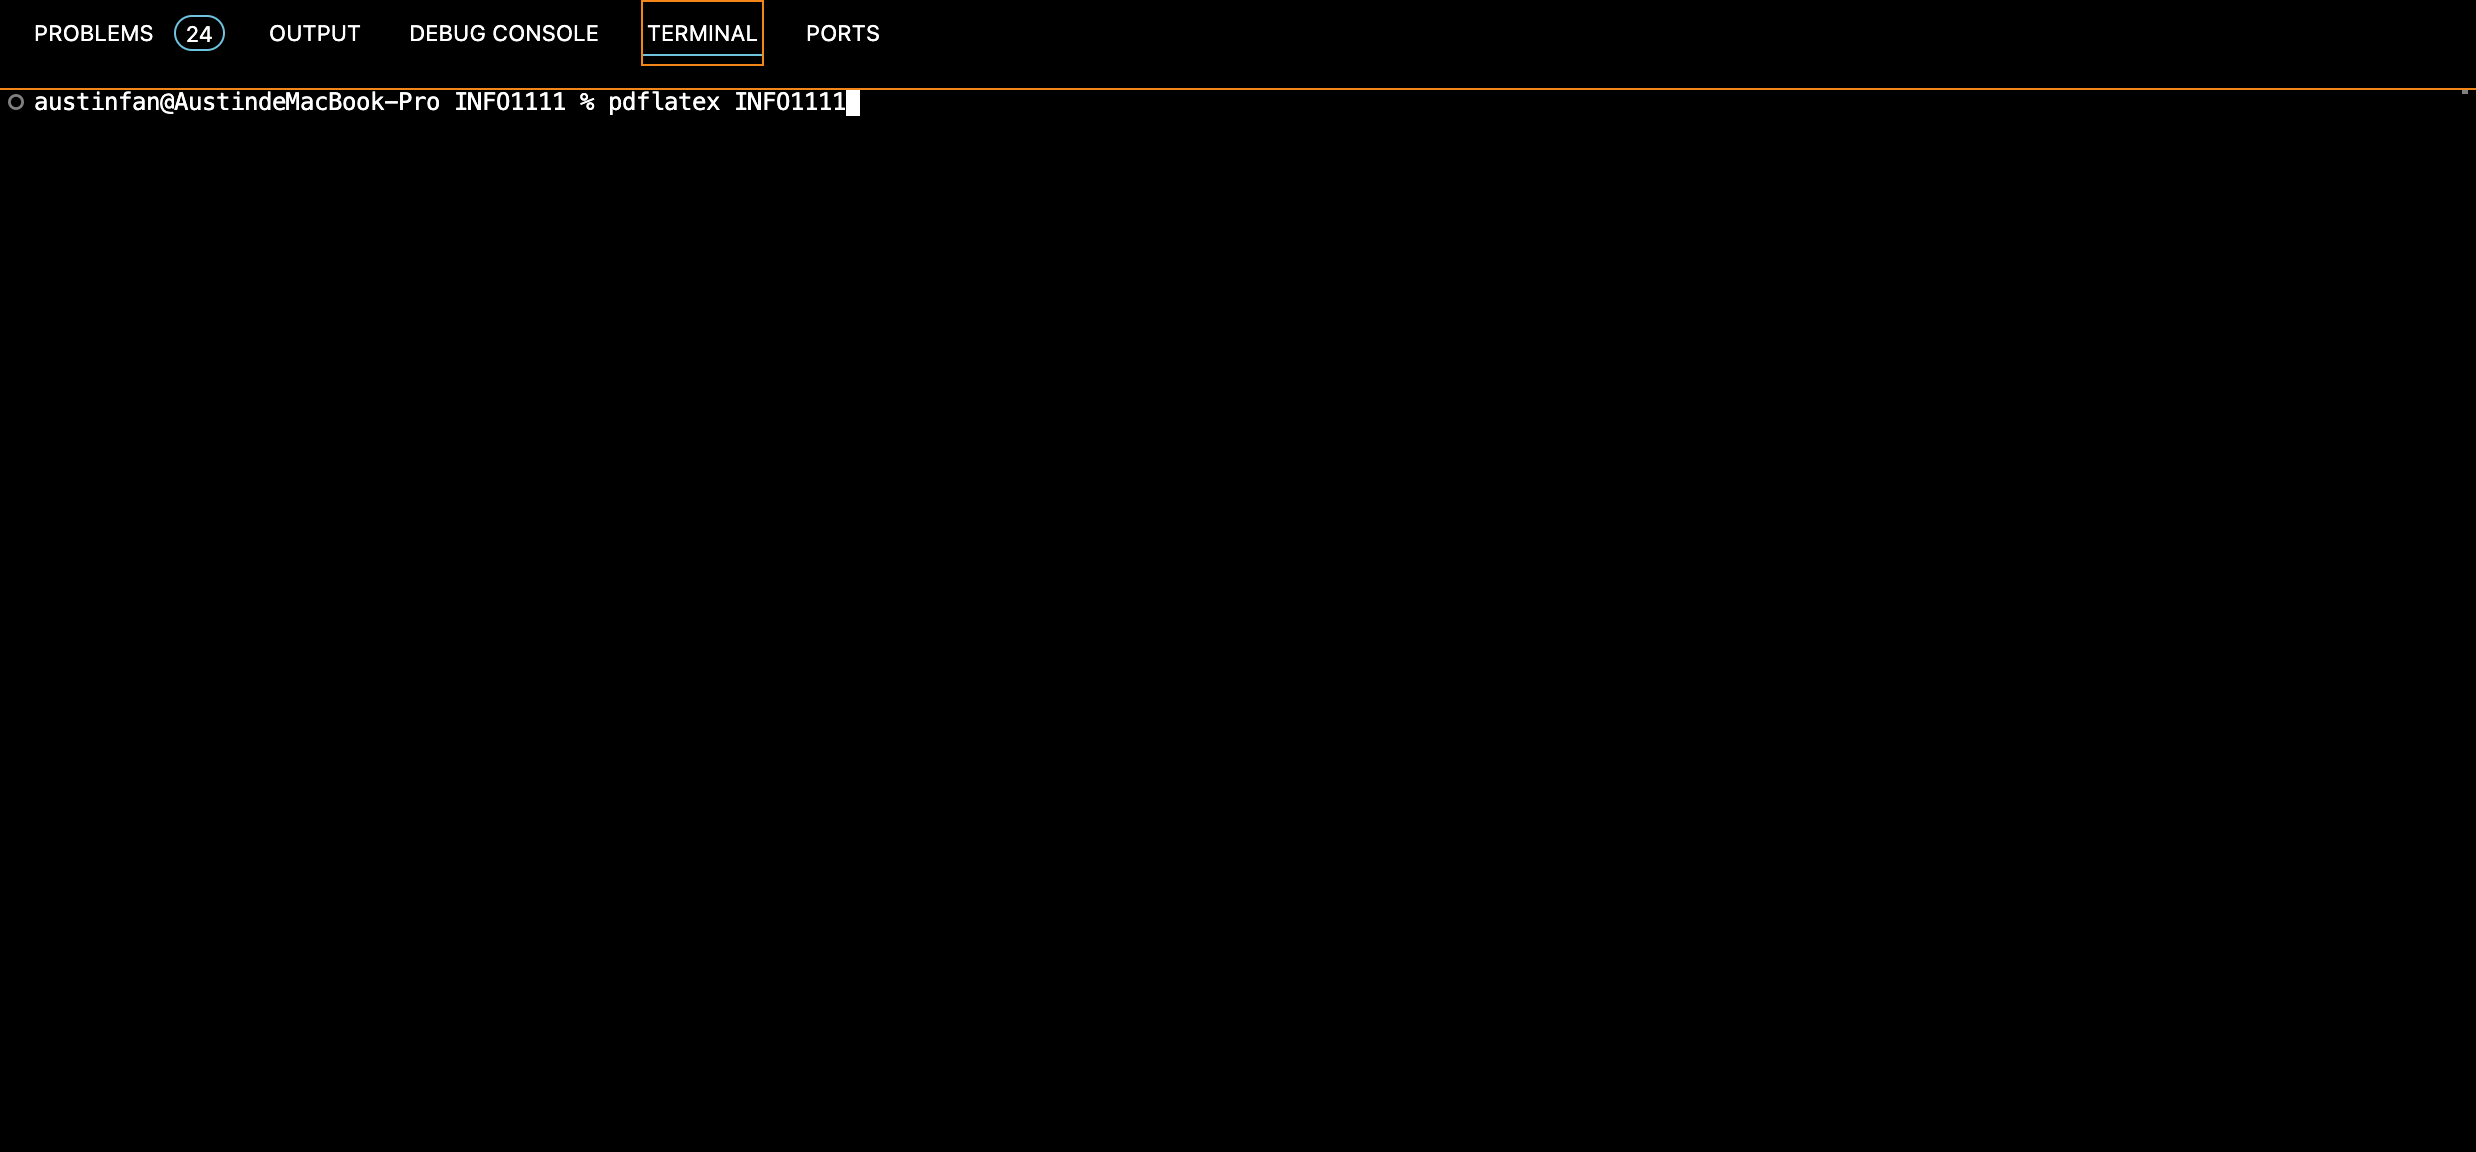
\includegraphics[width=0.7\textwidth]{com1}
    \caption{Creating pdf for first time and the aux file}
\end{figure*}

\begin{figure*}[H]
    \centering
    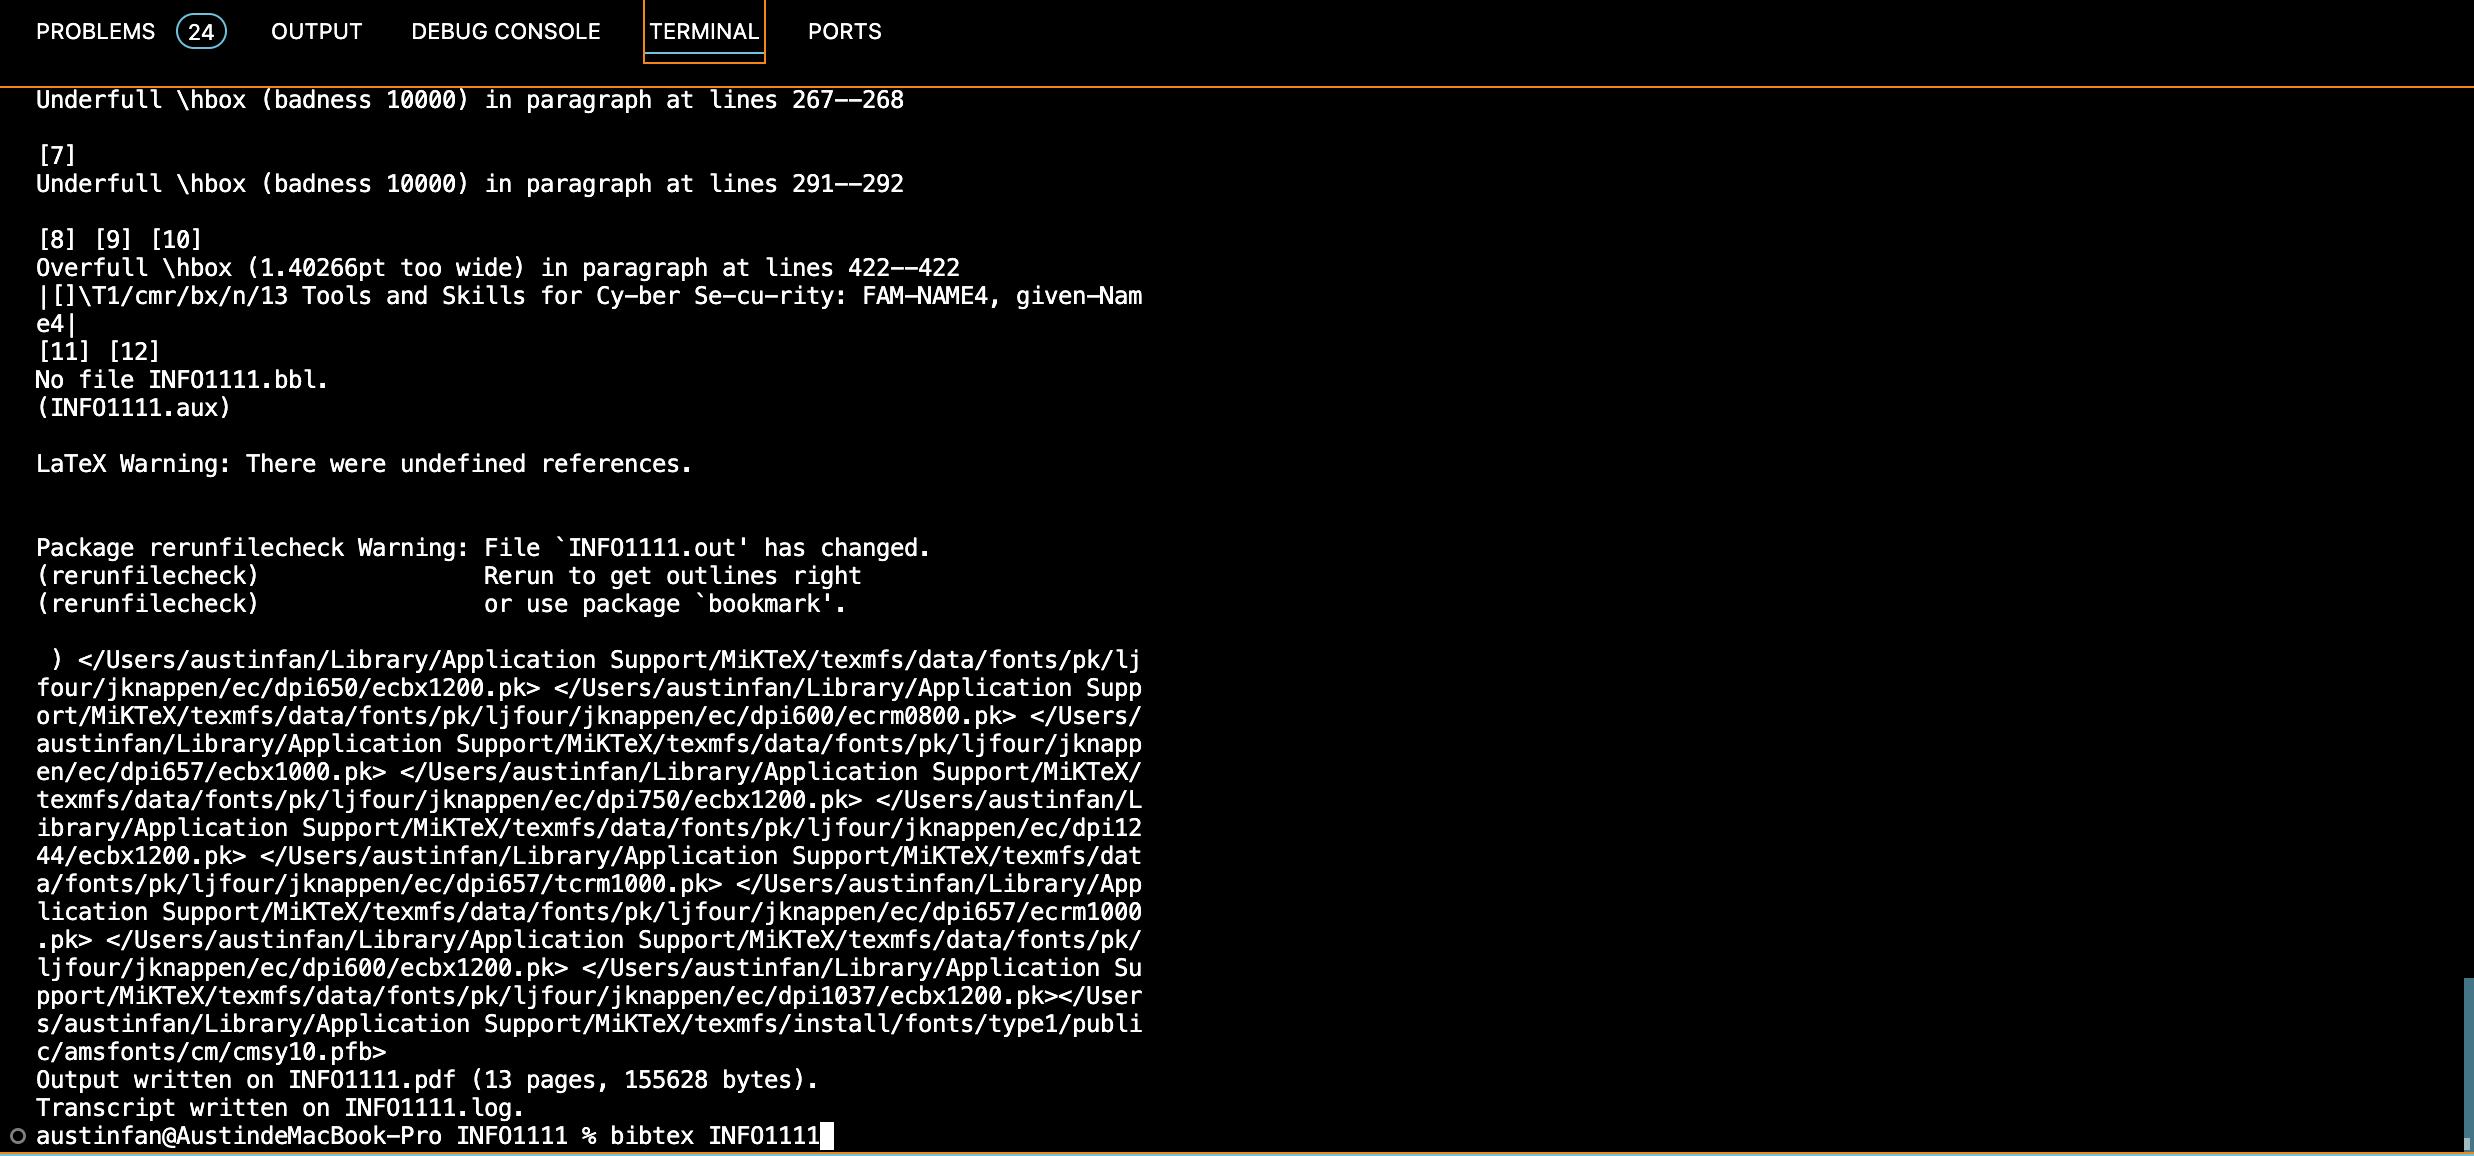
\includegraphics[width=0.7\textwidth]{com2}
    \caption{Creating the bbl file}
\end{figure*}

\begin{figure*}[H]
    \centering
    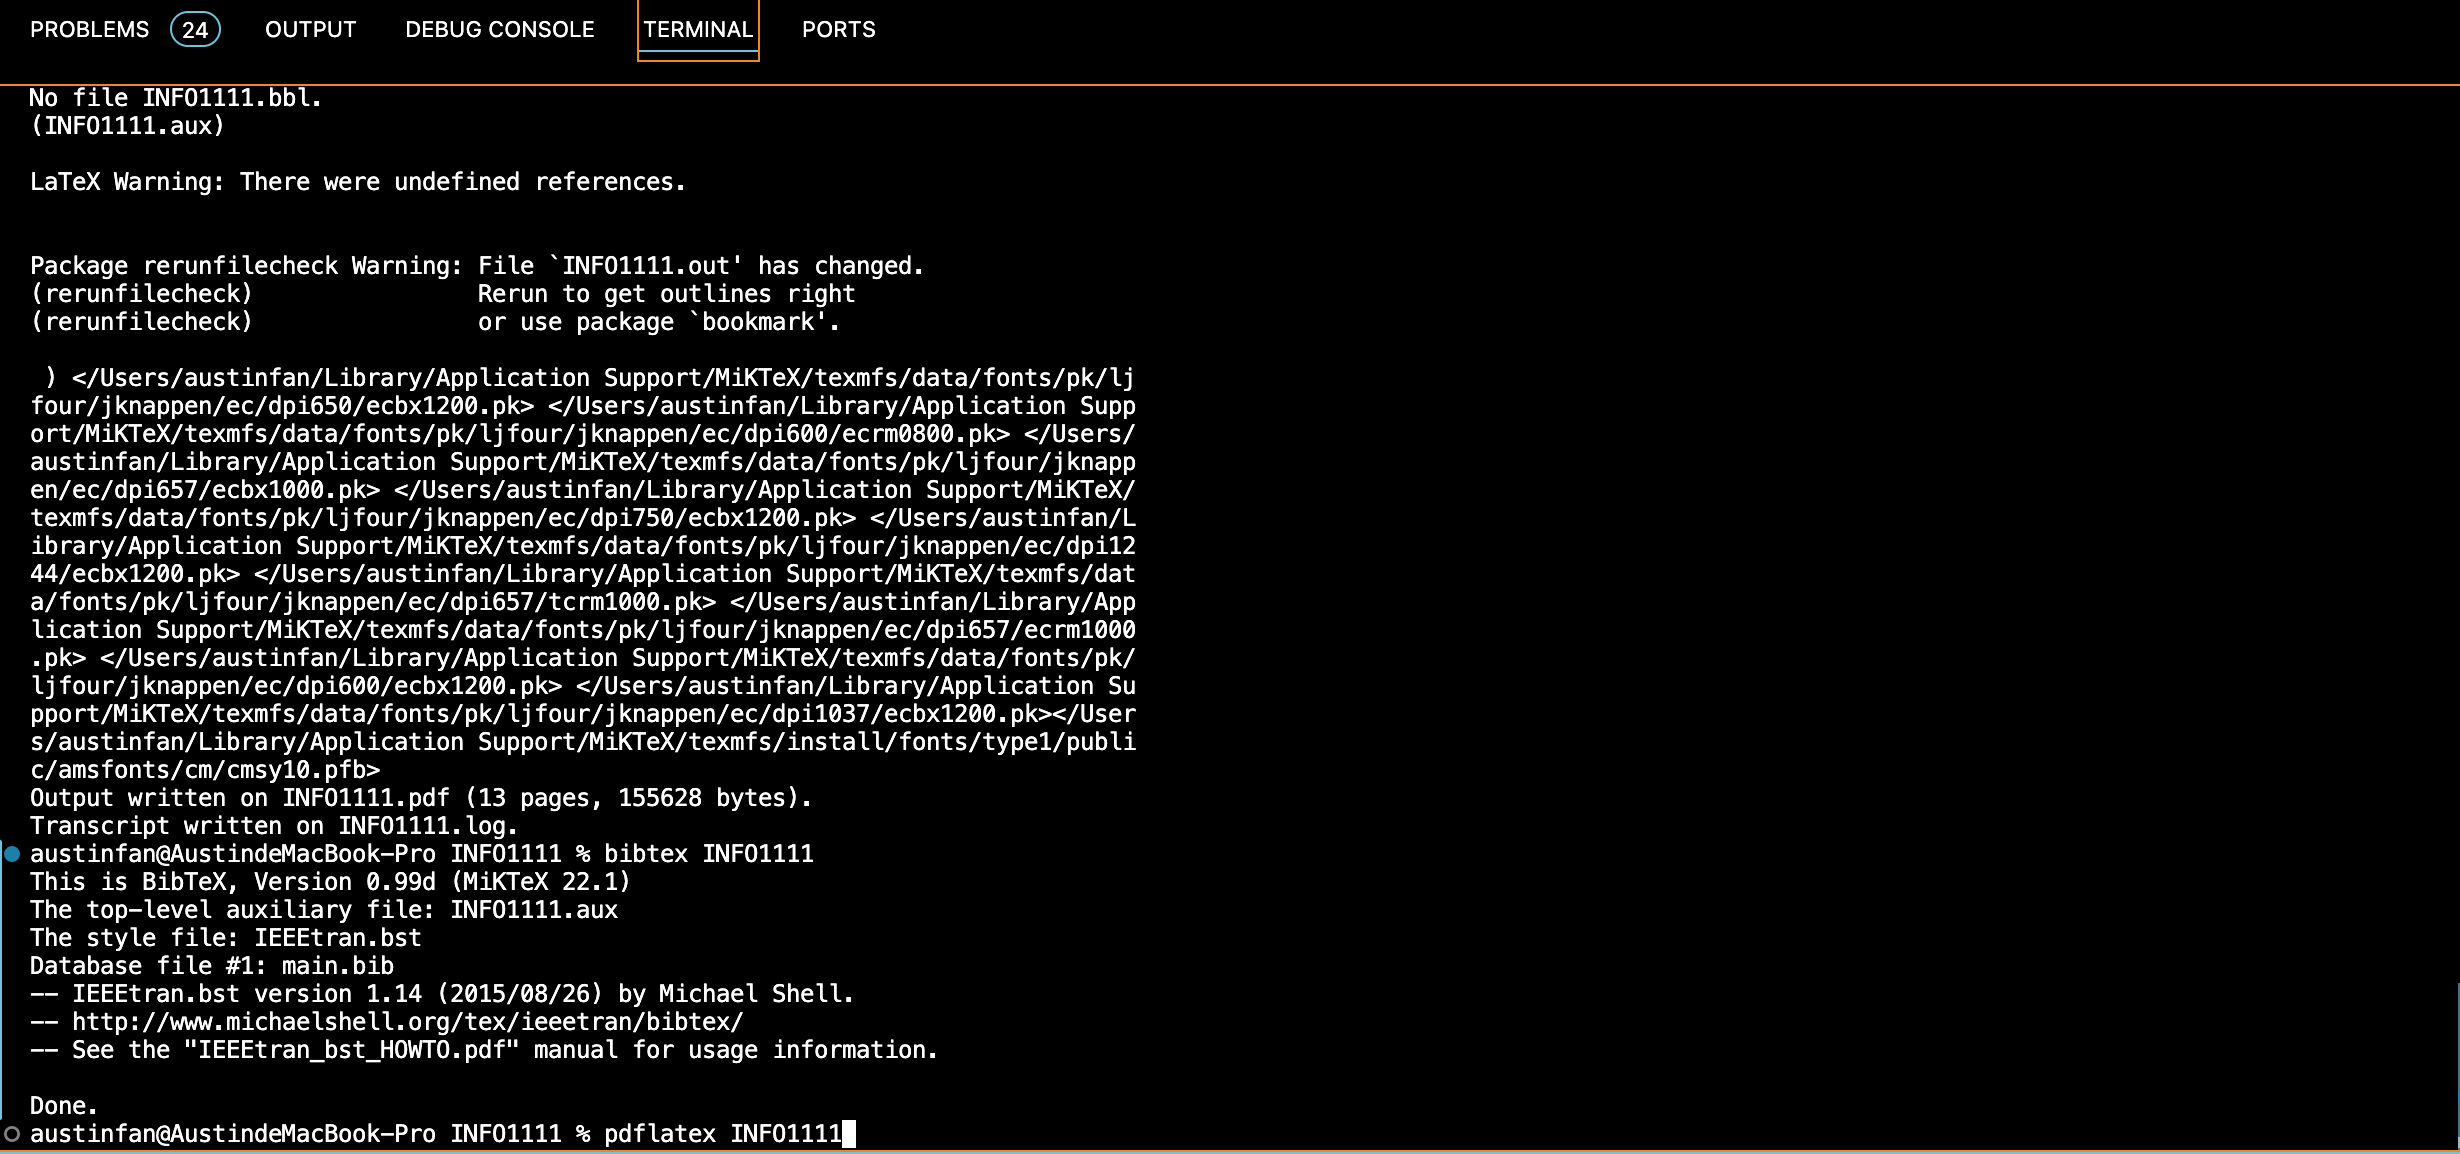
\includegraphics[width=0.7\textwidth]{com3}
    \caption{Creating pdf again with the bibliography}
\end{figure*}

\begin{figure*}[H]
    \centering
    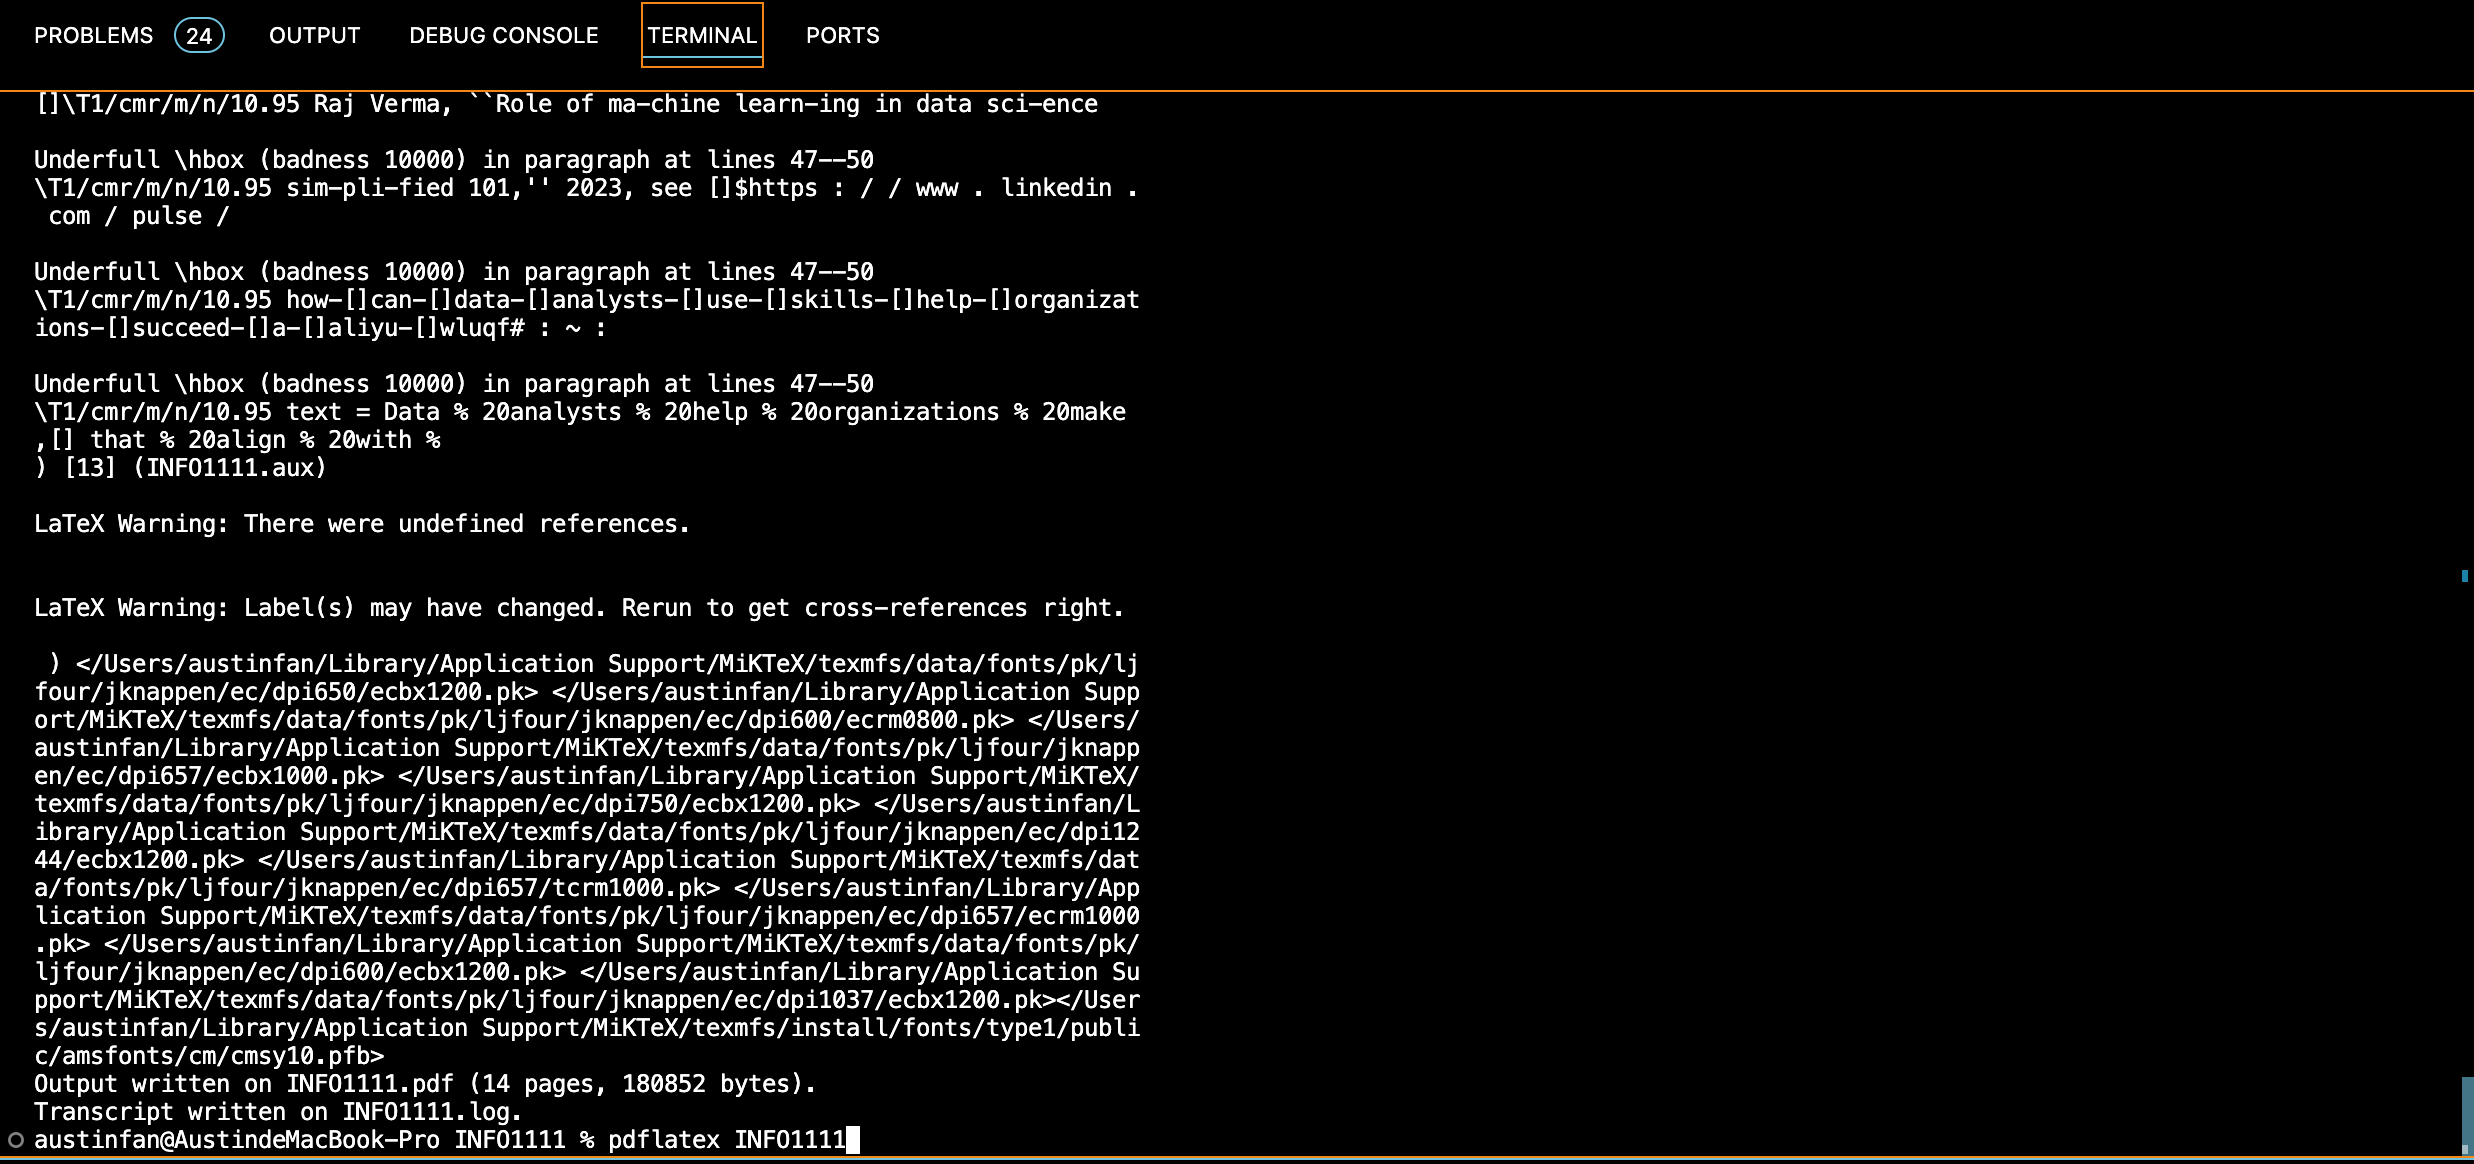
\includegraphics[width=0.7\textwidth]{com4}
    \caption{Creating the final pdf}
\end{figure*}

\begin{figure*}[H]
    \centering
    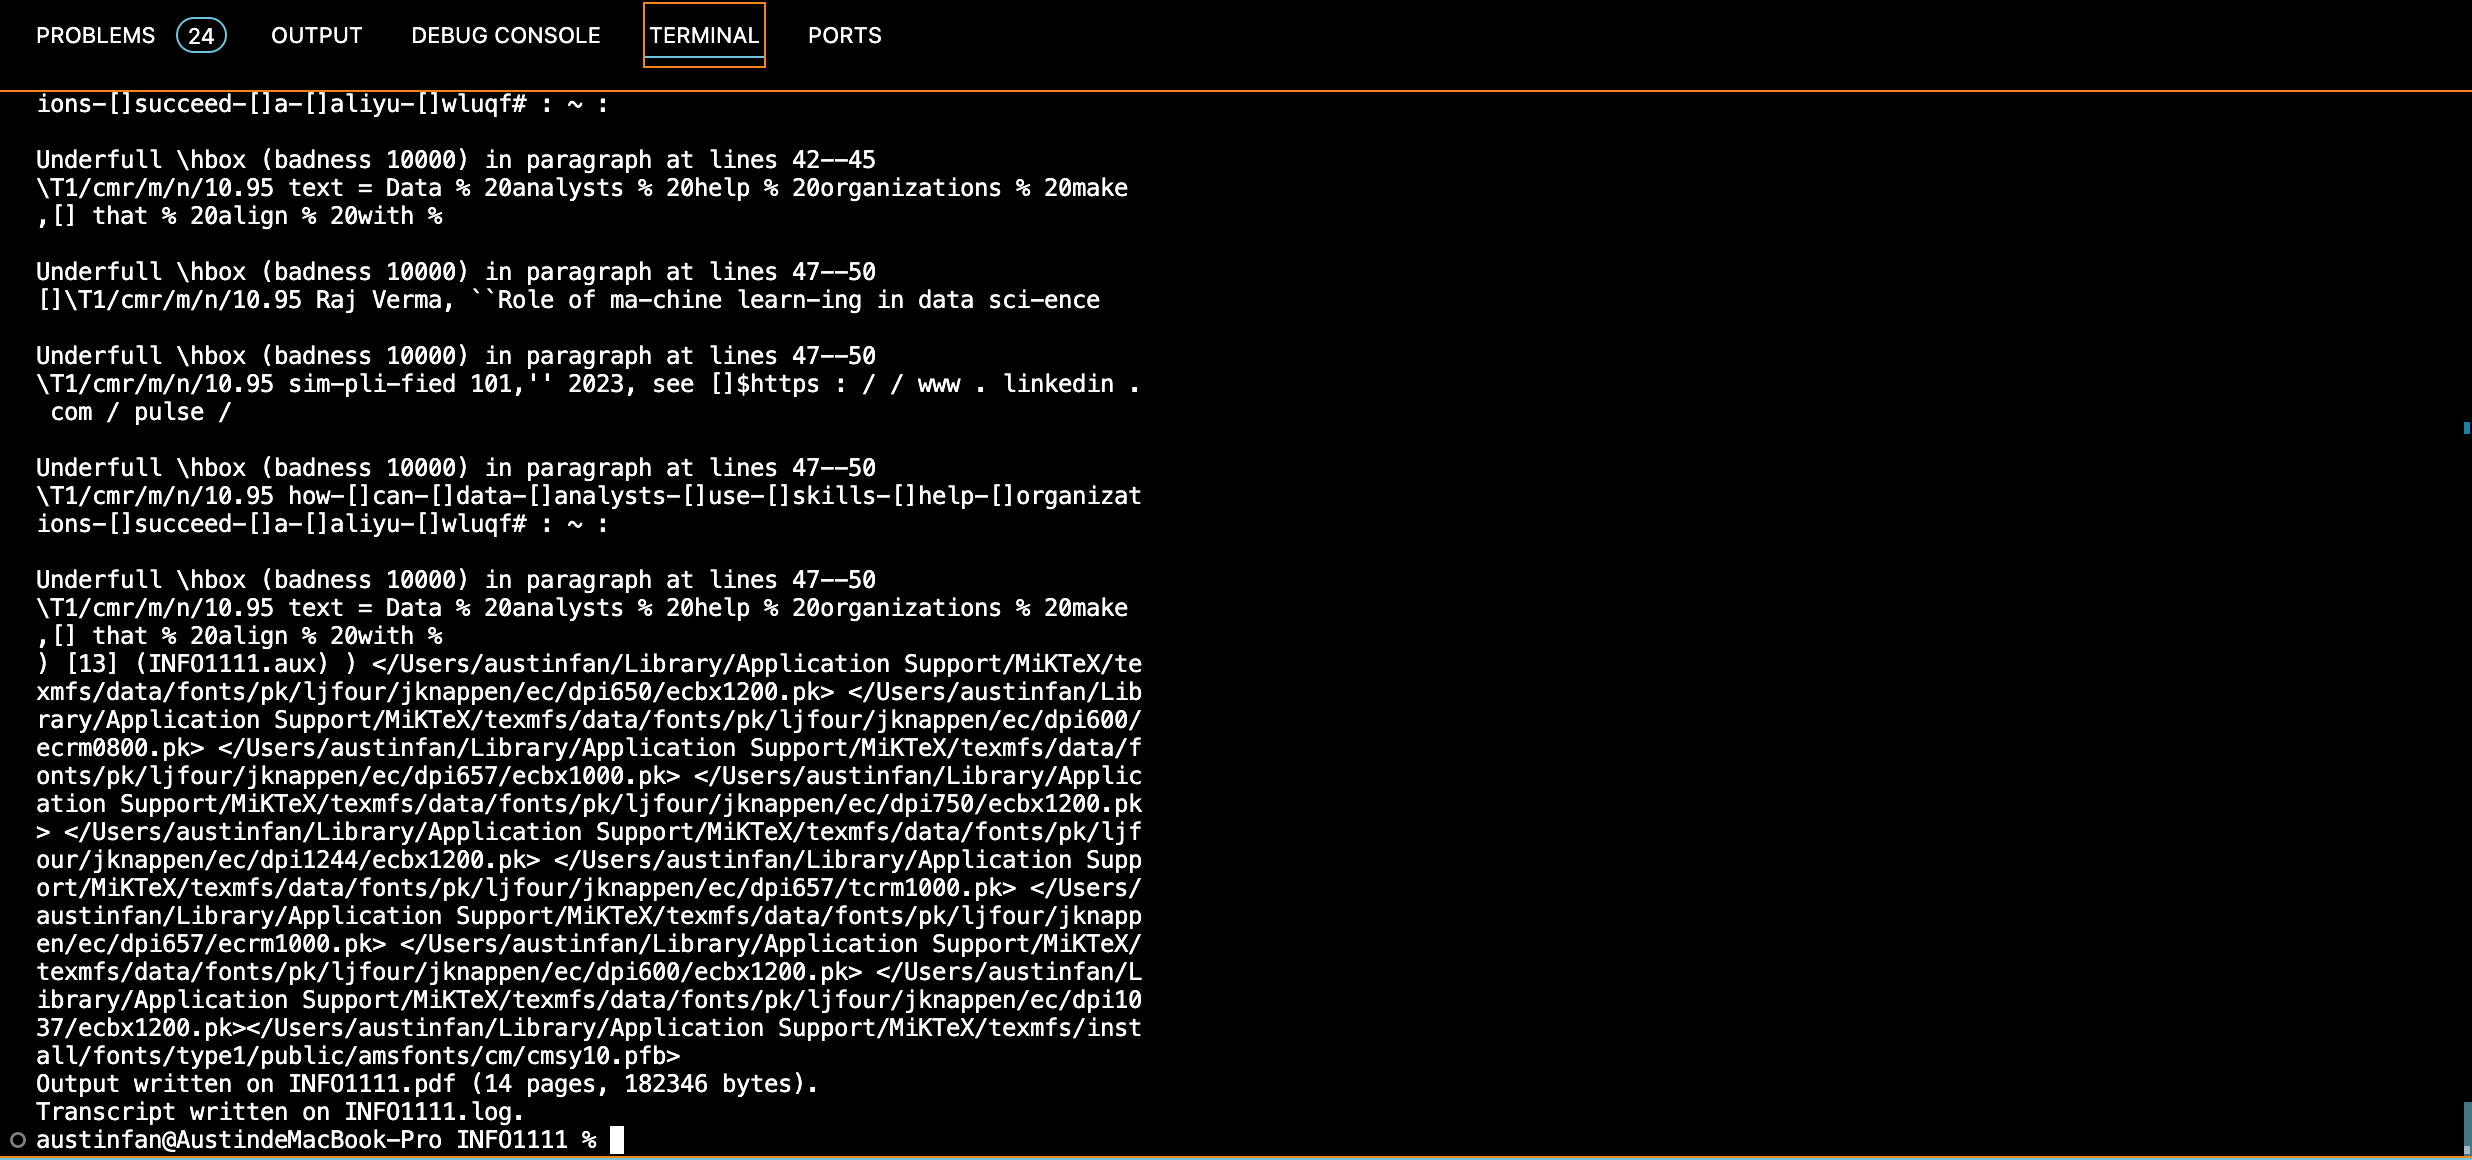
\includegraphics[width=0.7\textwidth]{com5}
    \caption{Output for previous command(Creating the Final pdf)}
\end{figure*}

\begin{figure*}[H]
    \centering
    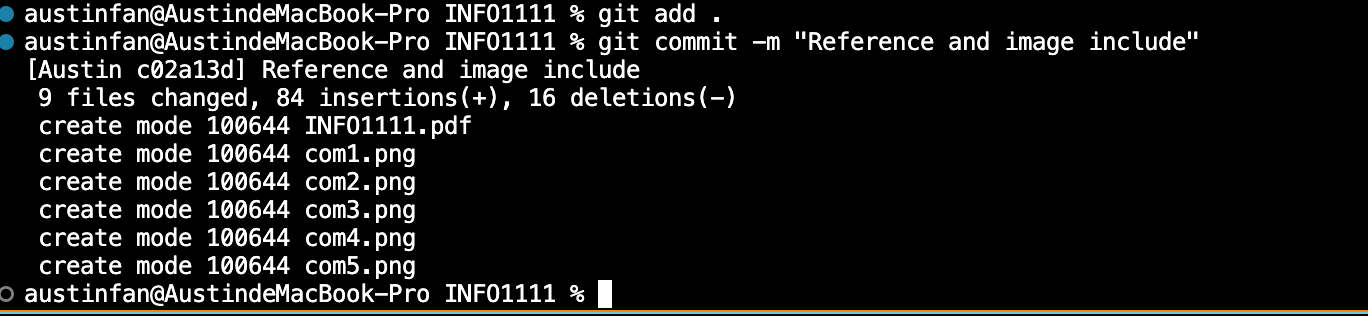
\includegraphics[width=0.7\textwidth]{git1}
    \caption{Commit to local repository}
\end{figure*}
% ========================================================
\newpage
\subsection{Skills for \majC: \studC}
\textbf{Programming/Software Development (PROG)}
\\[1em]
Programming proficiency is essential for software developers, most especially amidst rapidly evolving technologies present around us. Programming proficiency refers to one's ability to not only master multiple syntax of various programming languages but also to write clean and efficient code and algorithms. It is fundamental in developing a software developer's logical thinking and problem solving skills, enabling them to create effective and efficient solutions for complex tasks and meet client requirements.\cite{PROG3}\cite{PROG4}.
\\[1em]
High level programming skills also empower Software Developers to have adequate knowledge in utilizing relevant tools and frameworks that can not only enhance code quality but also provide assurance in its level of correctness. Examples include facilitating peer code review and refactoring. These allow software developers to develop a bug-free consistent and effective system \cite{PROG1}\cite{PROG3}. 
\\[1em]
Overall, mastering the fundamentals of programming is essential as it allows developers to quickly adapt to new tools and languages present in the field. This expertise is also beneficial in the development aspect of projects as the team's programming proficiently is integral in creating competitive and high quality software products that meet the stakeholders’ requirements. Moreover, this skill serves as the basic foundation for other important skills such as Software Design and Testing \cite{PROG1}\cite{PROG3}.
\\[1em]
\\[1em]
\noindent \textbf {Software Design (SWDN)} 
\\[1em]
According to Computer.org, software design is integral in the creation process of  standards-compliant software and serves as the blueprint for most existing software systems.  It is the process where Software developers conceptualize and identify the architectural framework and platform that the software is going to be built upon \cite{SWDN1}.
\\[1em]
 Adept knowledge and skills in implementing various software design techniques and principles is crucial in a software developer’s ability to create and maintain a reliable, modifiable, scalable and reusable software application \cite{SWDN1}\cite{SWDN2}. This technical skill enables developers to meet client-defined requirements with the most optimal and cost-effective high level designs. Proficient software design skill prevents significant system and functional flaws stemming from ineffective initial software design, avoiding potentially costly consequences for firms.\cite{SWDN1}
\\[1em]
\\[1em]
\noindent \textbf {Testing (TEST)}
\\[1em]
Testing serves as the backbone of reliability, completeness and efficiency for developed software systems. It is an important skill that gives software developers a gauge of how well the developed software meets the client’s requirements in terms of the software’s functionality, security, stress and performance etc.\cite{TEST1}  Tests help enhance the development process by allowing developers to detect functional and non-functional issues early on, thereby preventing escalation of the problem that could lead to costly rework.\cite{TEST2}\cite{TEST3}.
\\[1em]
Other testing methods also take into account feedback from user experiences in using the software. This provides developers with important insights that ultimately influence their development direction. Furthermore, tests also give developers an evaluation of the overall software design in terms of quality of the product, integration and compatibility with other software systems.
\cite{TEST2}.
\\[1em]
\\[1em]
Screenshots for terminal commands and output, showing compiling and uploading of local repository on to github. 
\begin{figure*}[H]
    \centering
    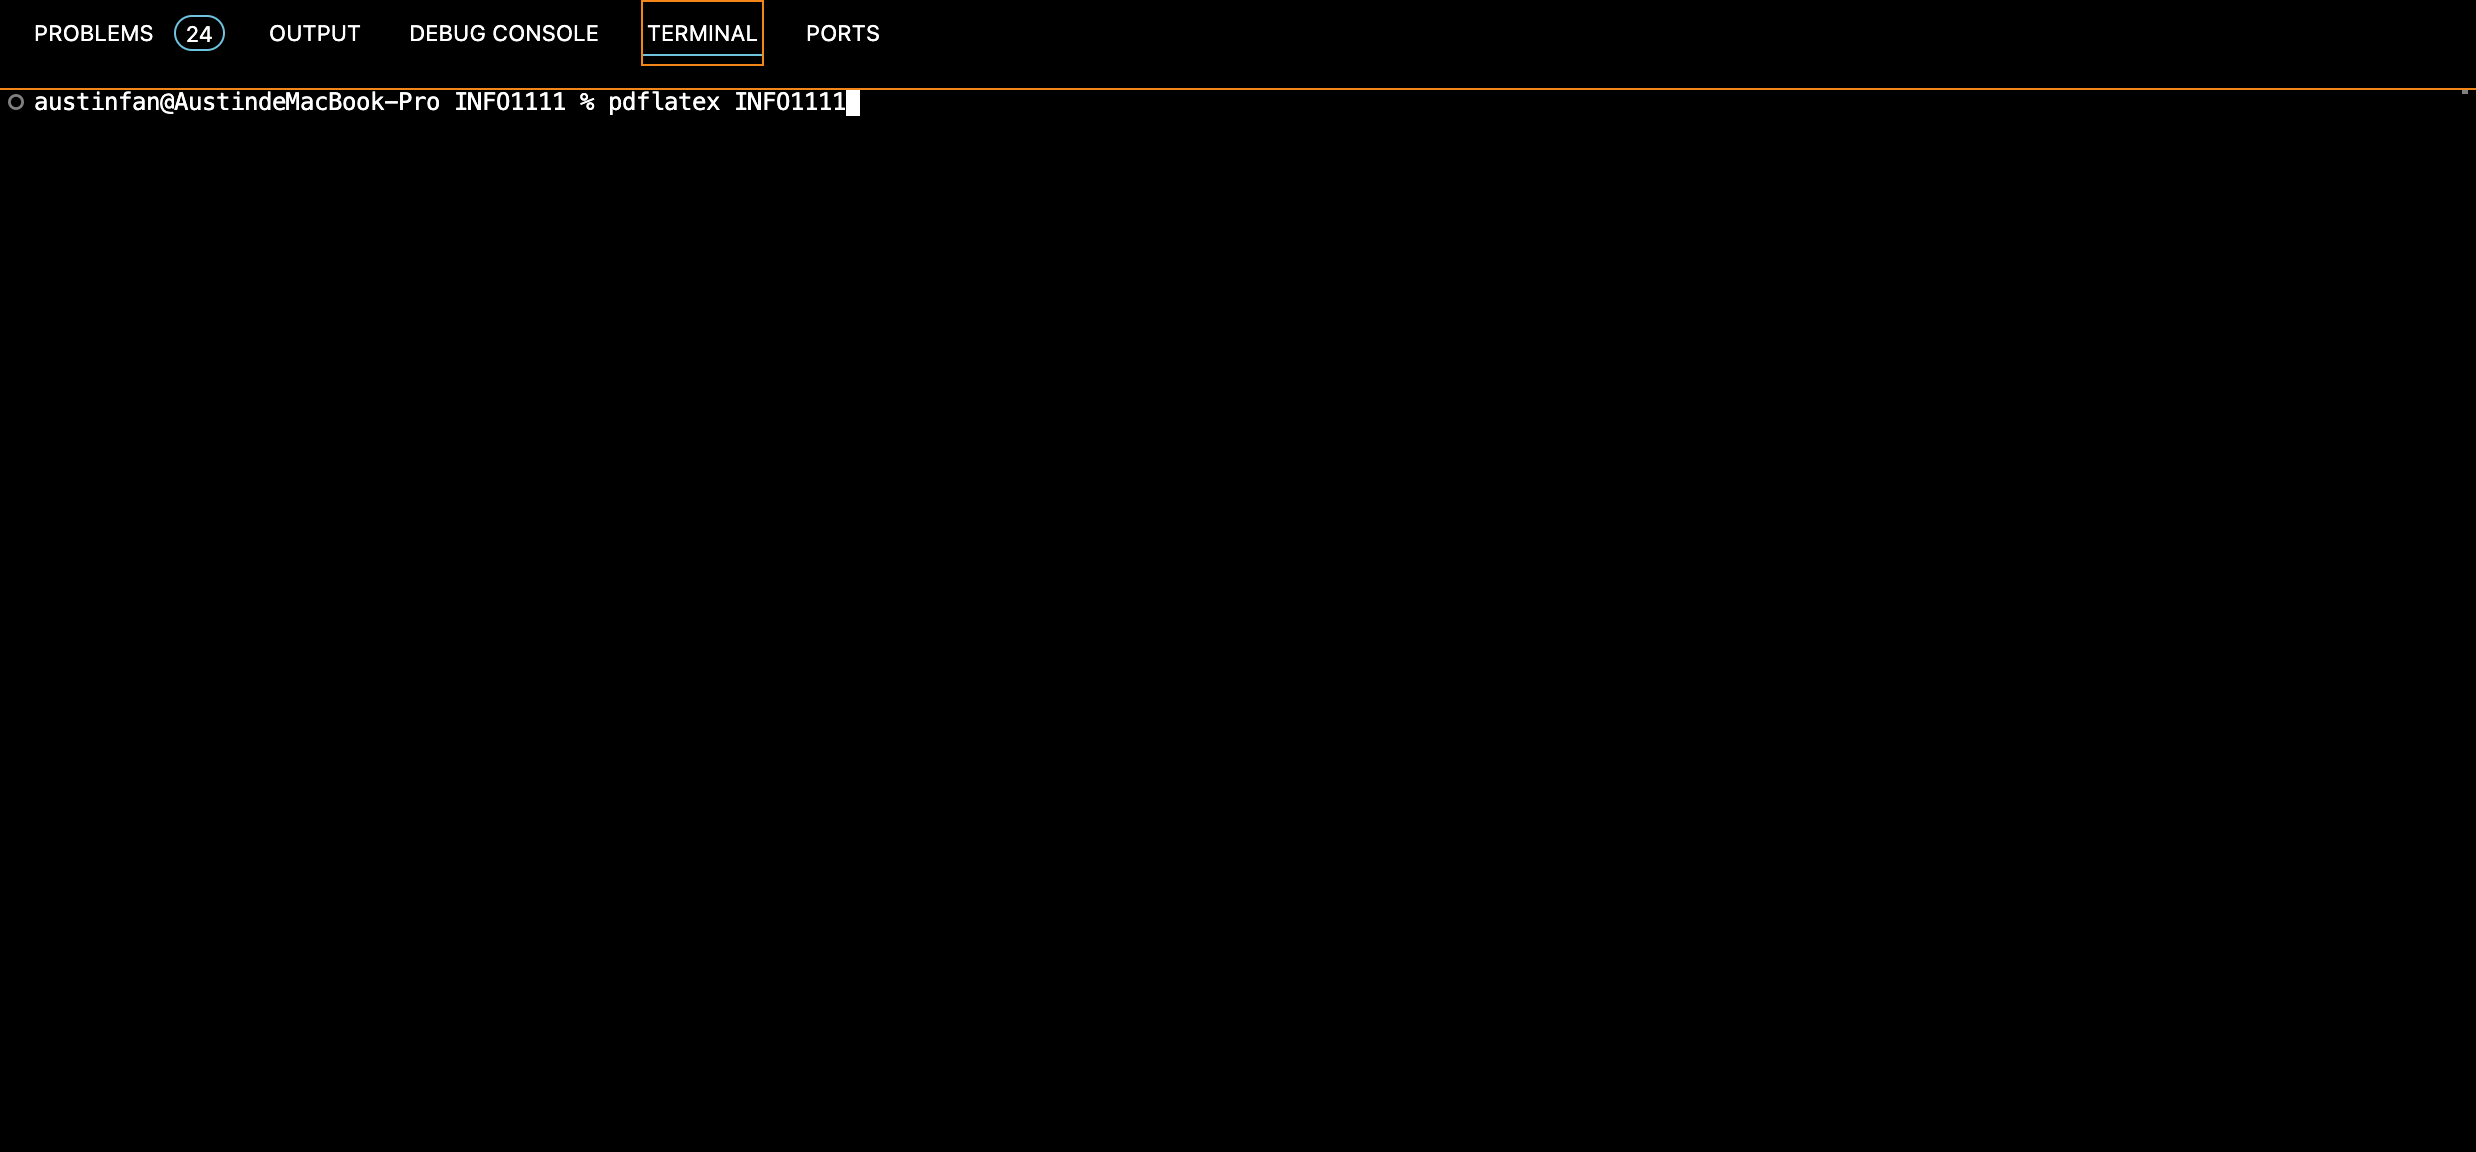
\includegraphics[width=0.7\textwidth]{com1}
    \caption{Creating pdf for first time and the aux file}
\end{figure*}

\begin{figure*}[H]
    \centering
    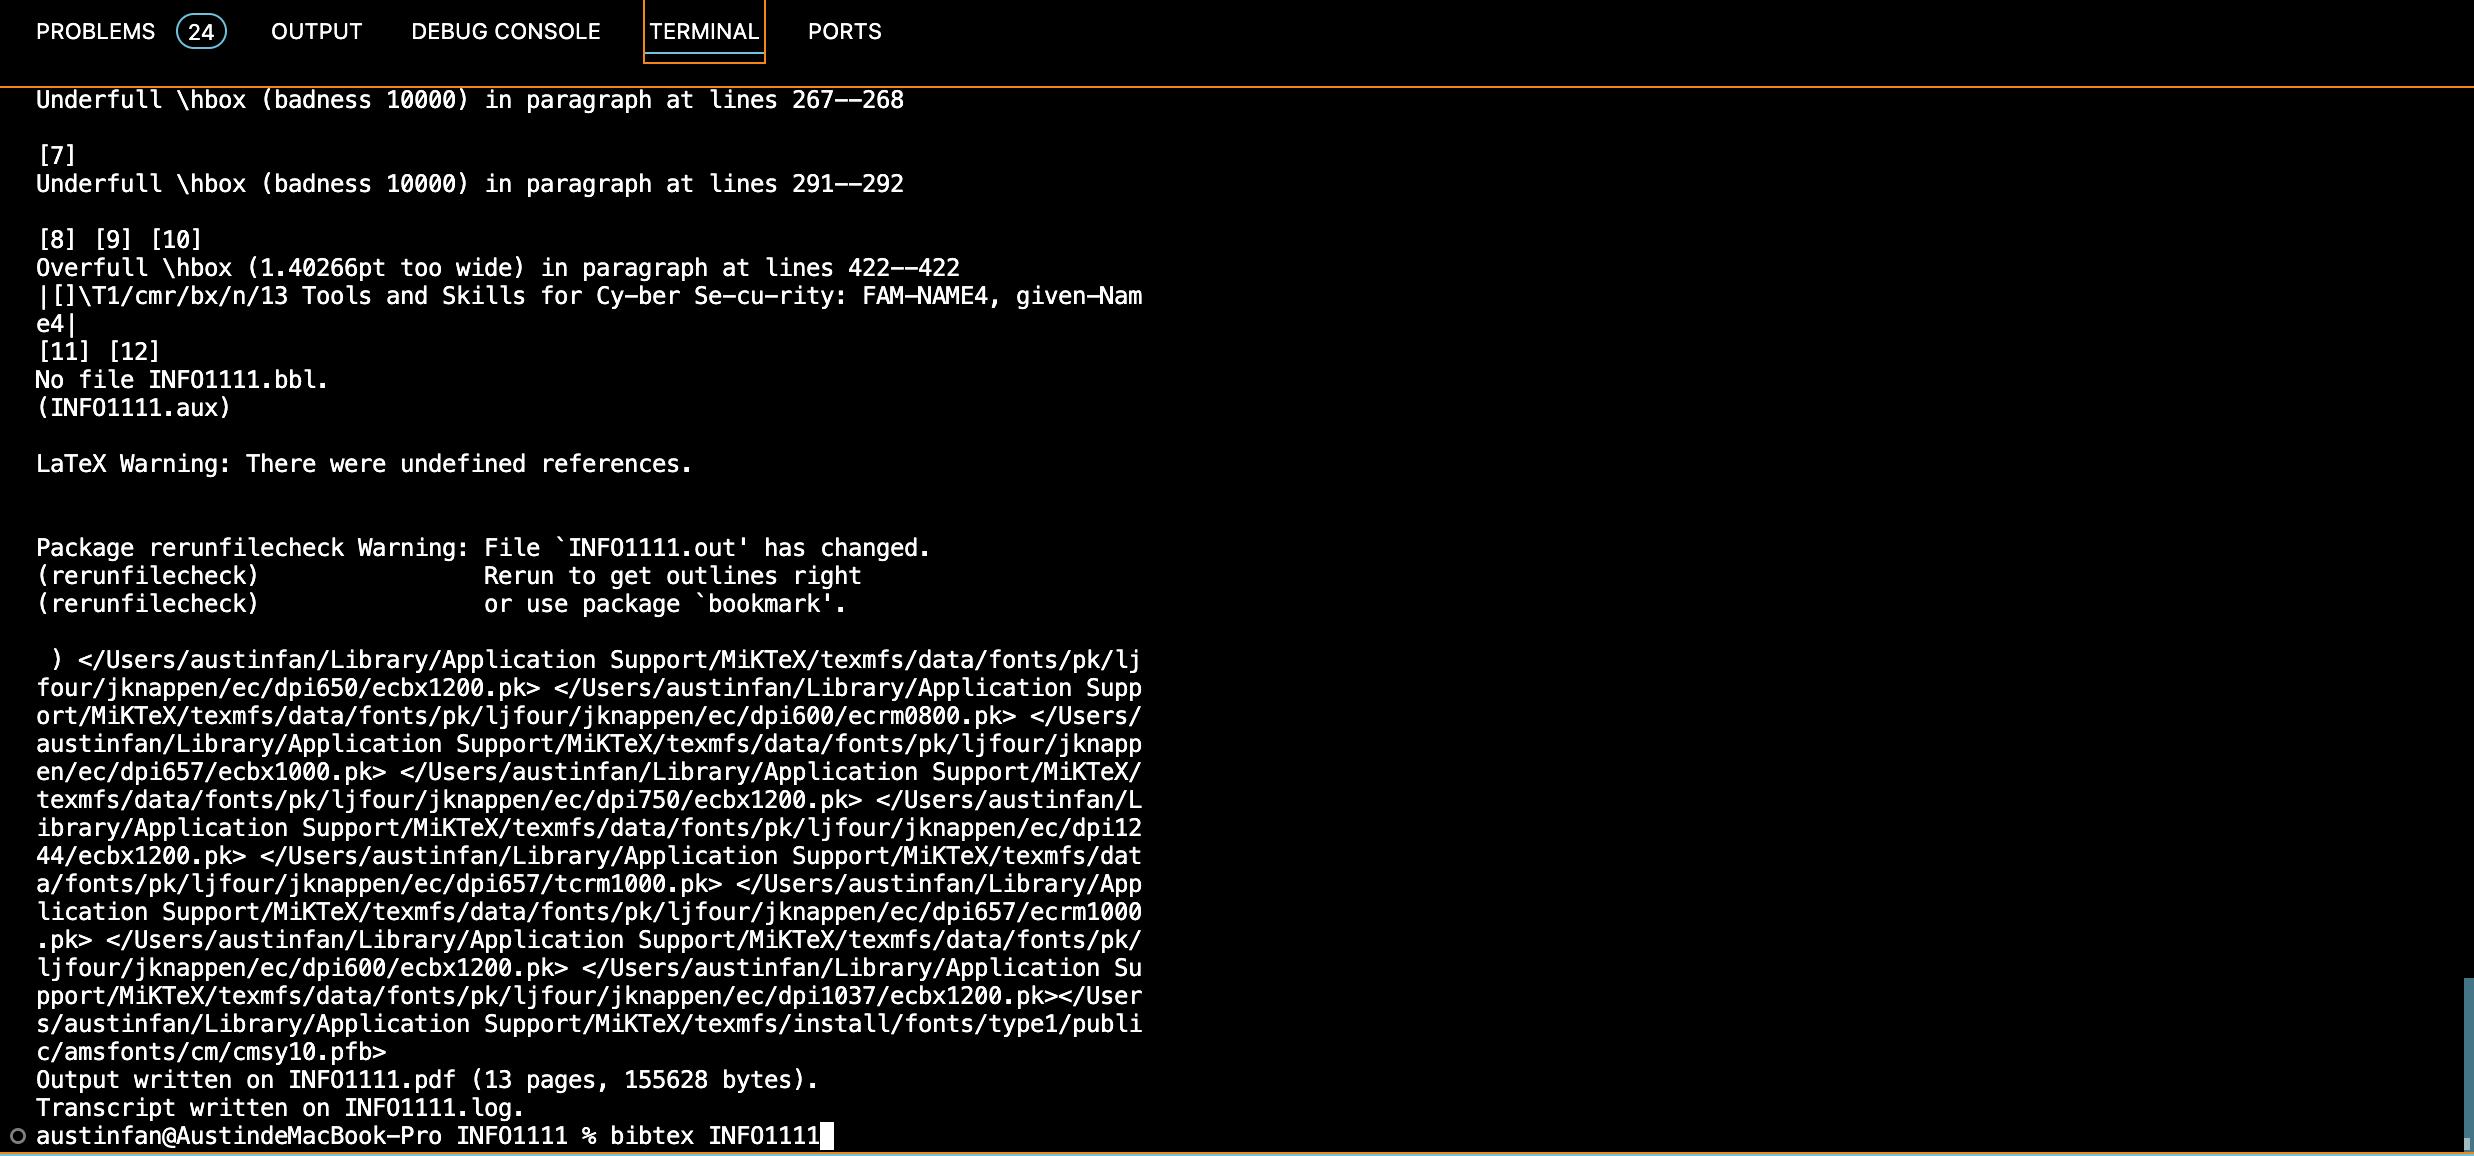
\includegraphics[width=0.7\textwidth]{com2}
    \caption{Creating the bbl file}
\end{figure*}

\begin{figure*}[H]
    \centering
    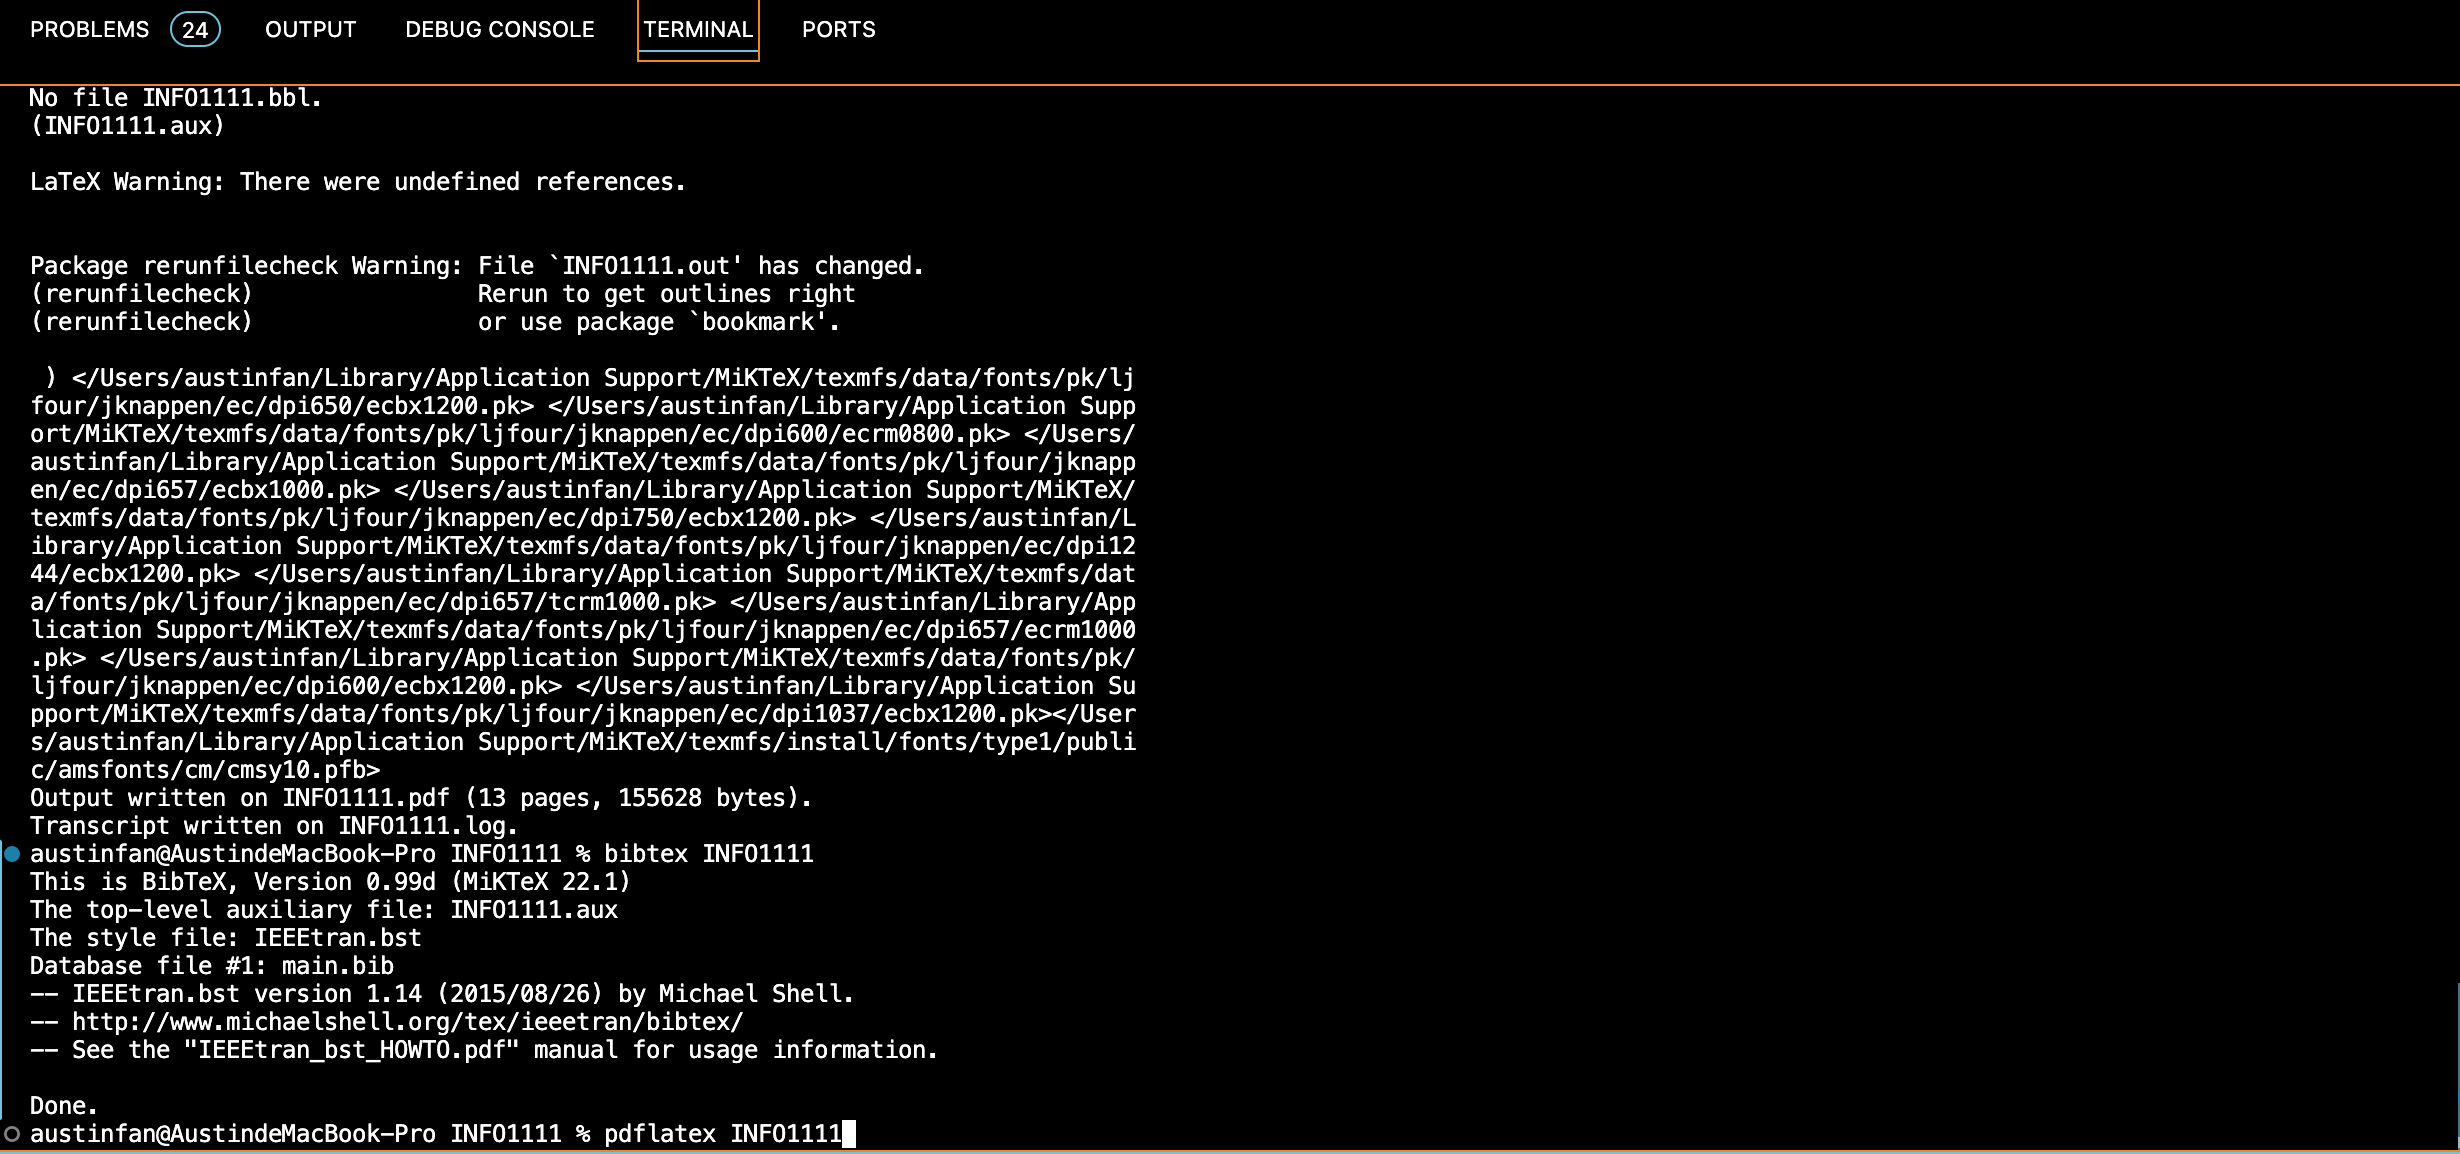
\includegraphics[width=0.7\textwidth]{com3}
    \caption{Creating pdf again with the bibliography}
\end{figure*}

\begin{figure*}[H]
    \centering
    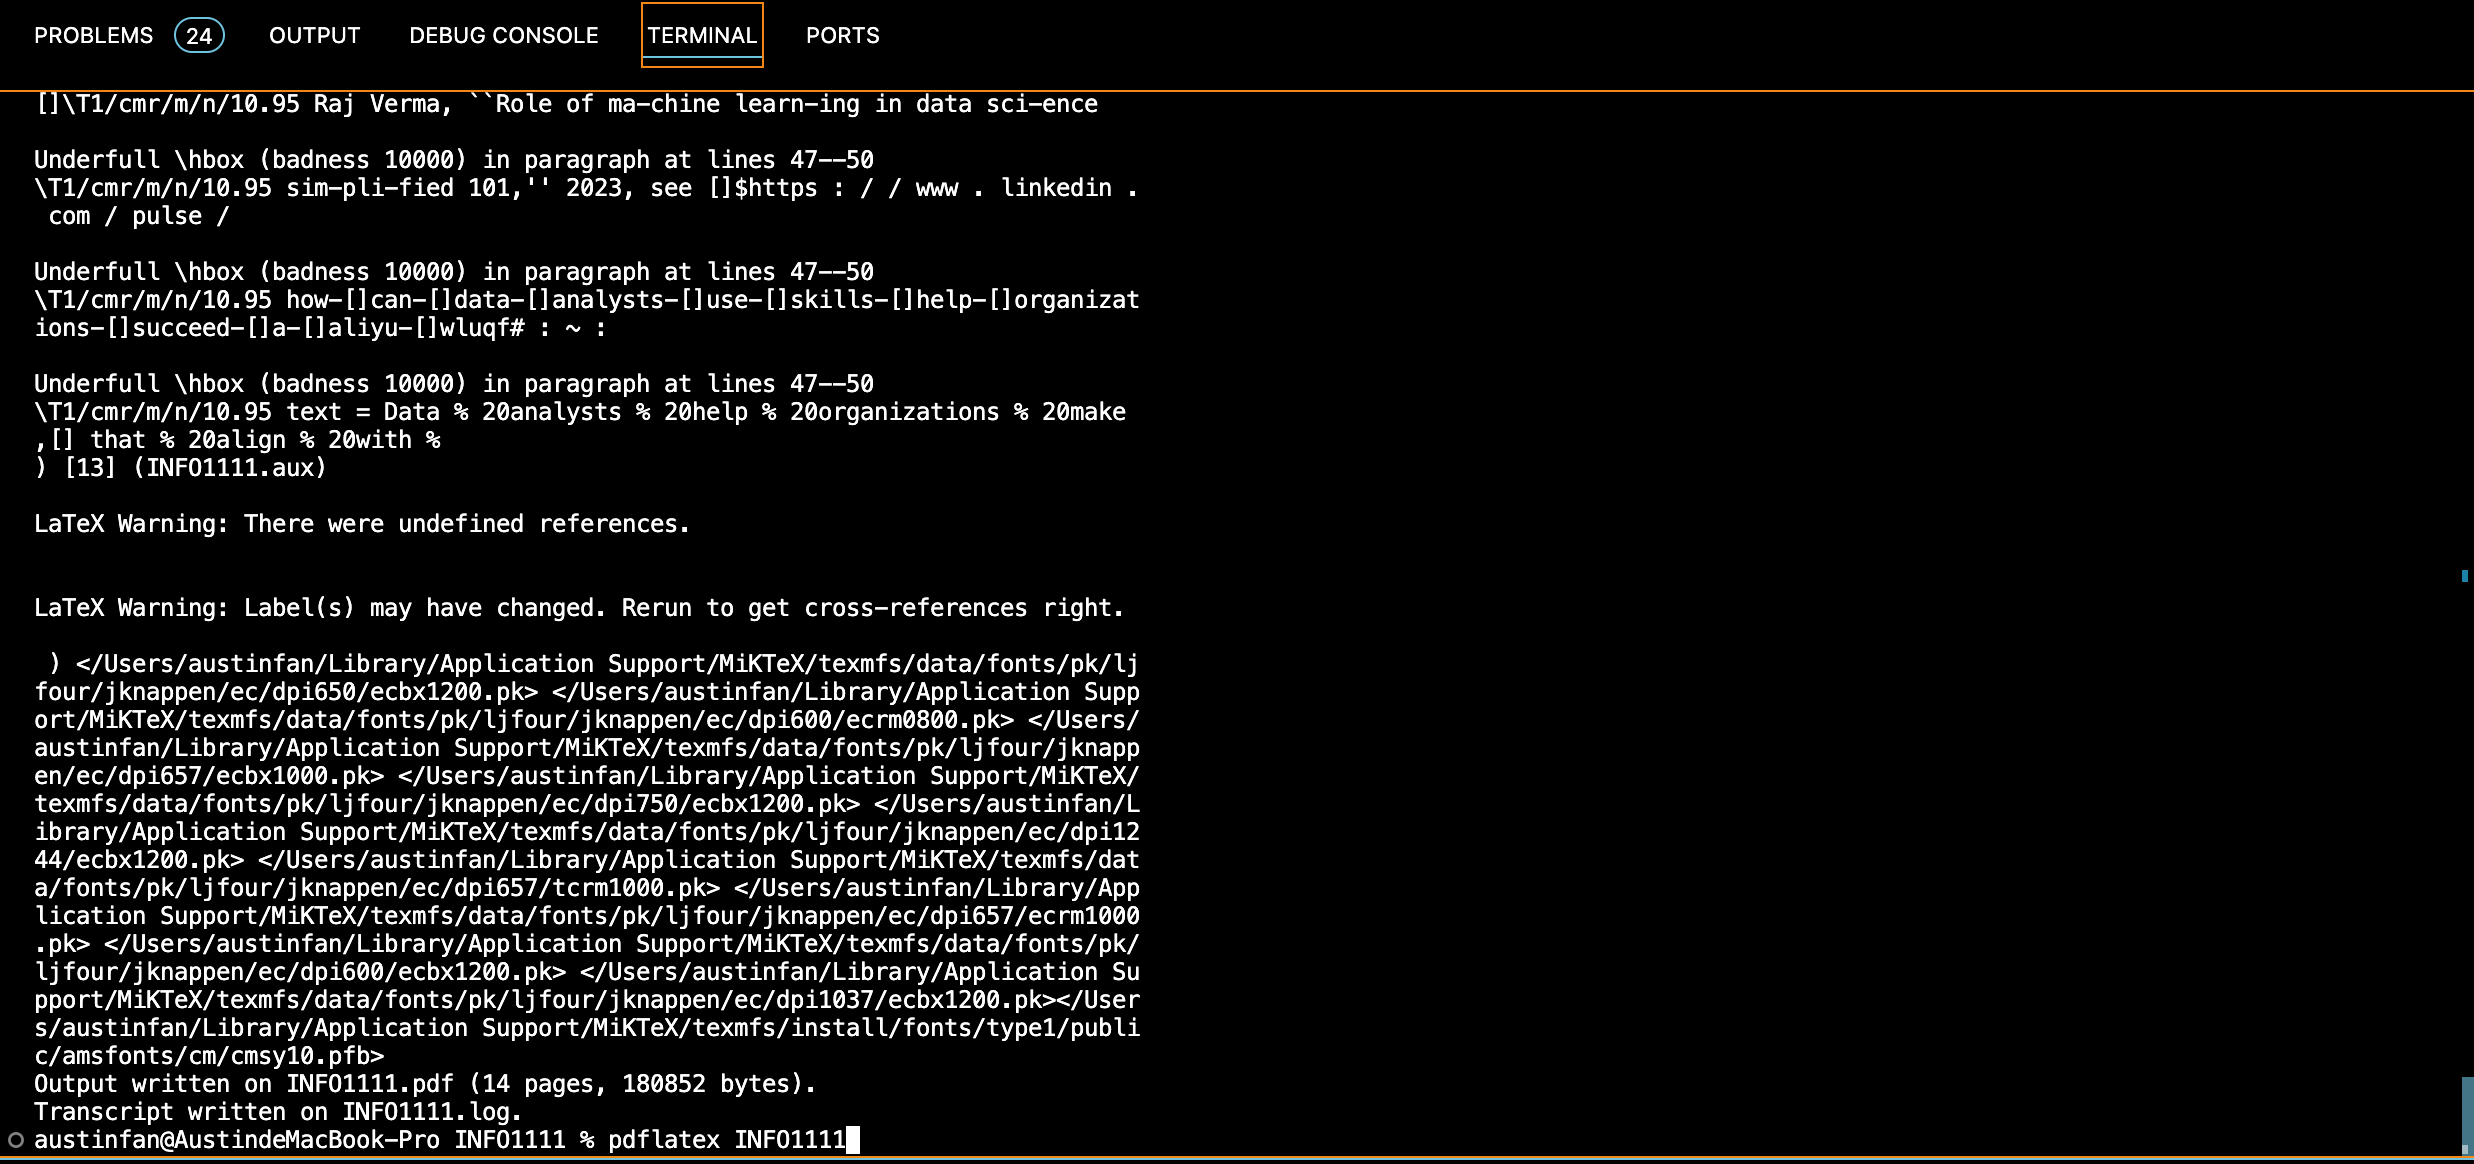
\includegraphics[width=0.7\textwidth]{com4}
    \caption{Creating the final pdf}
\end{figure*}

\begin{figure*}[H]
    \centering
    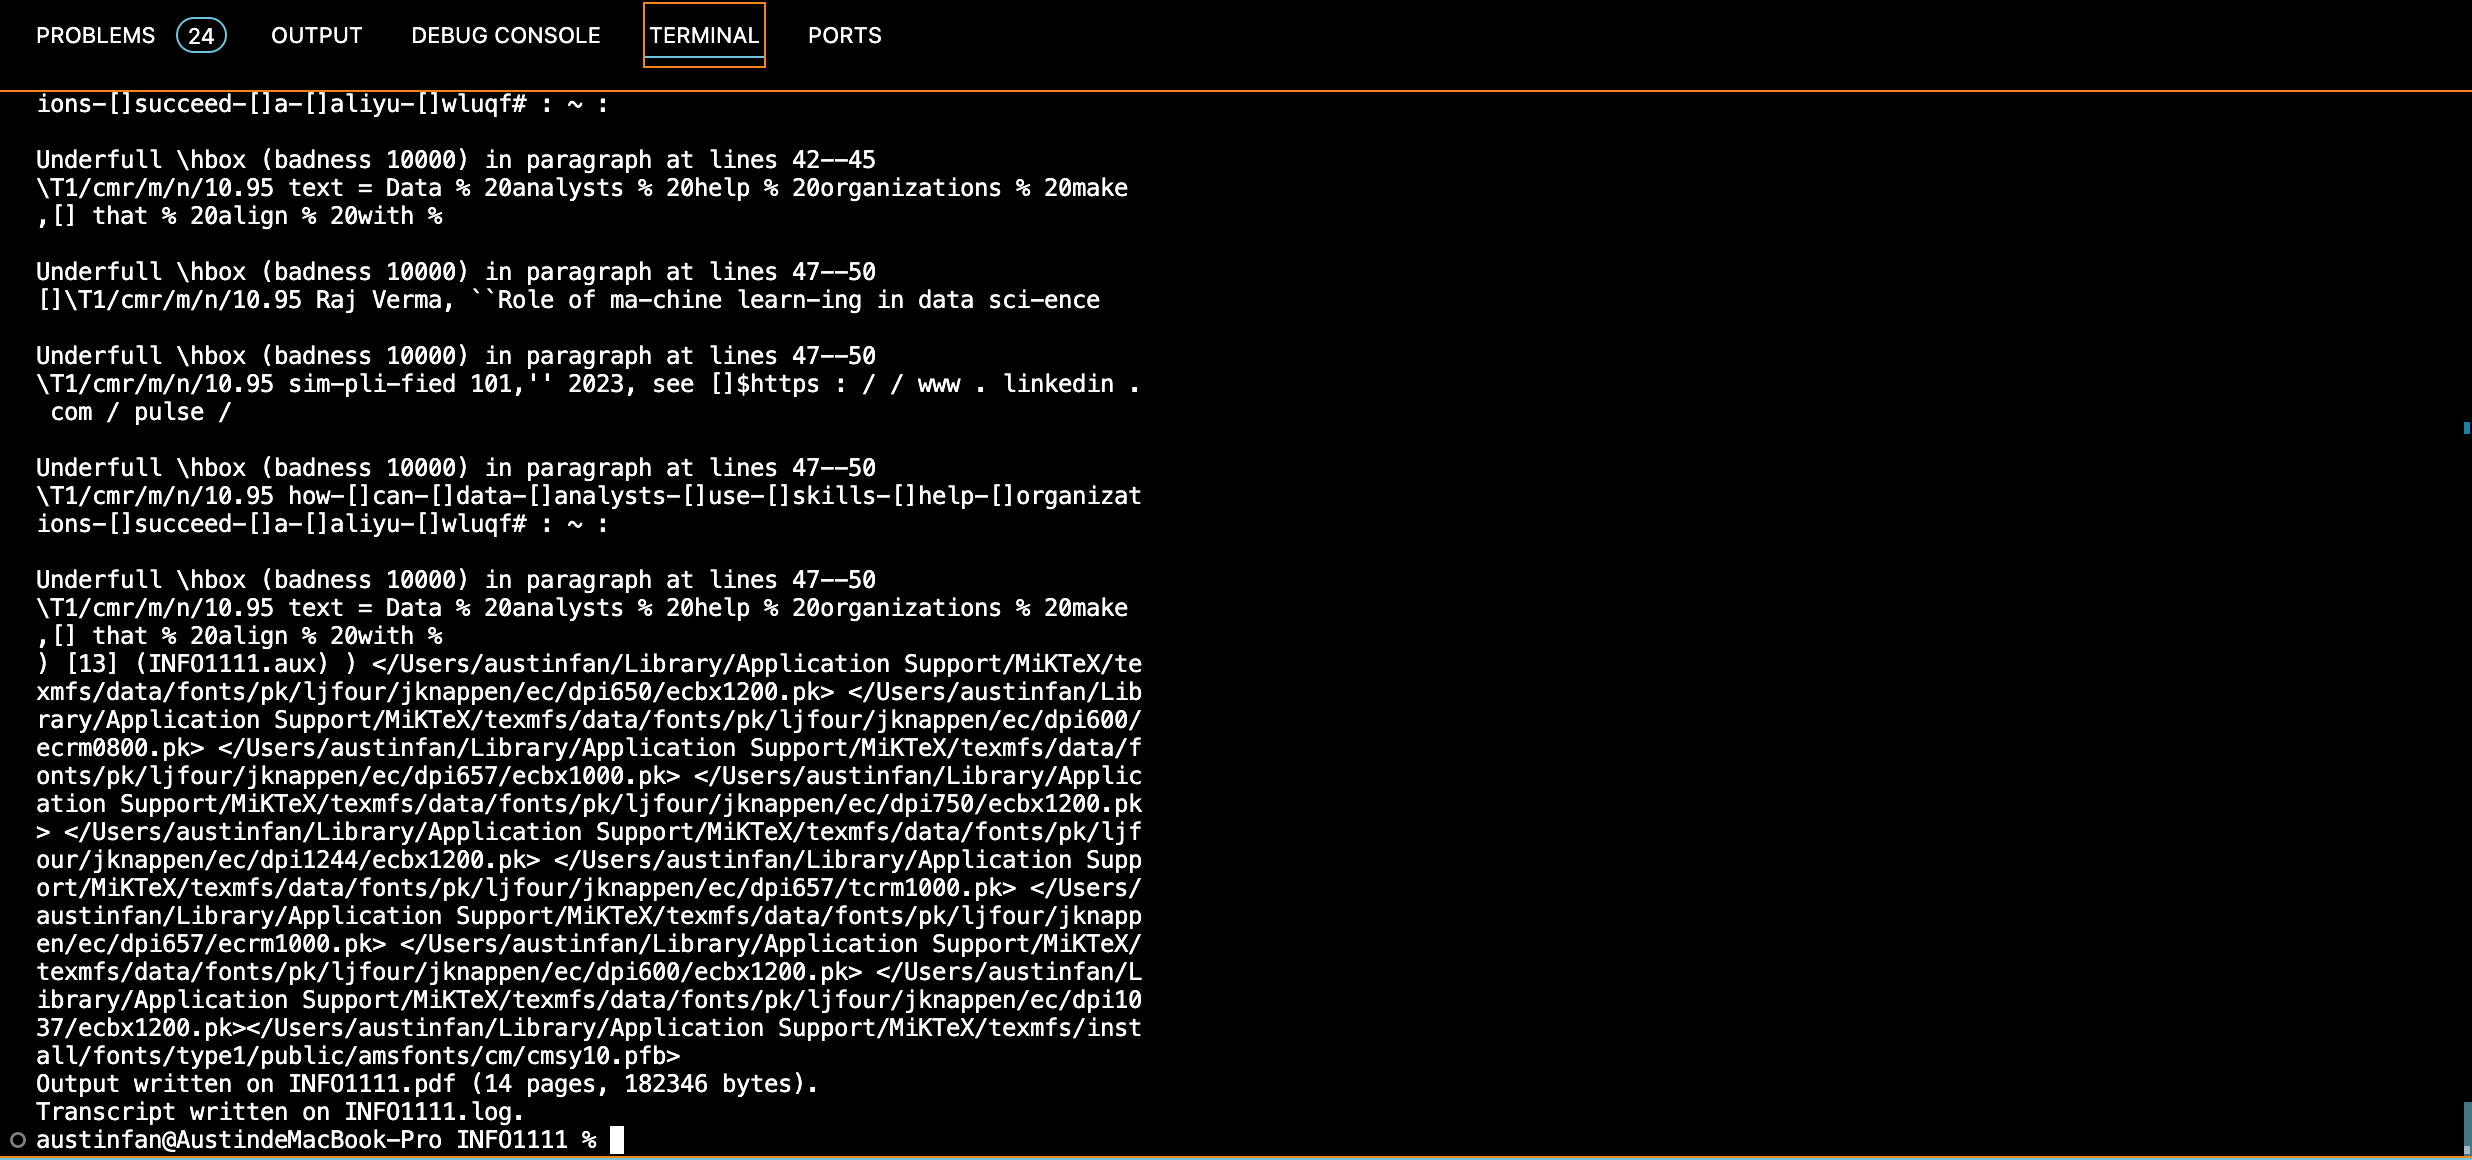
\includegraphics[width=0.7\textwidth]{com5}
    \caption{Output for previous command(Creating the Final pdf)}
\end{figure*}

\begin{figure*}[H]
    \centering
    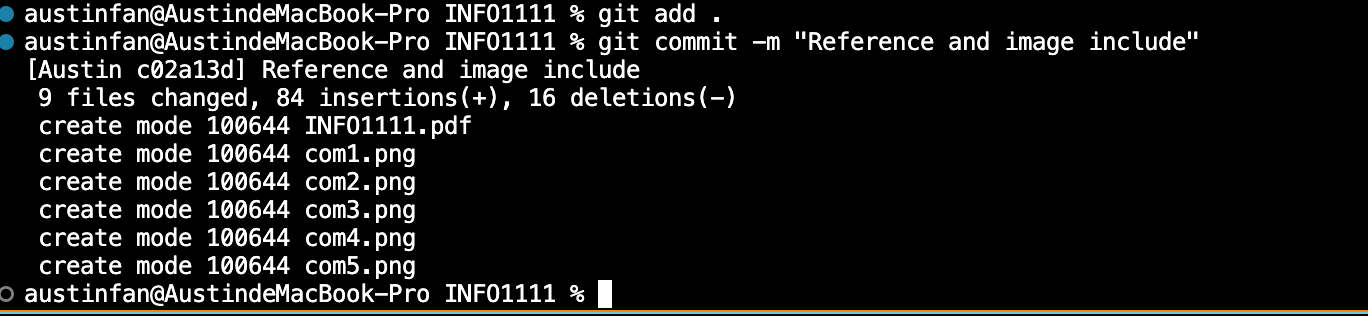
\includegraphics[width=0.7\textwidth]{git1}
    \caption{Commit to local repository}
\end{figure*}

%=======================================================================================

\newpage
\section{Submission contribution overview}

For each submission, outline the approach taken to your teamwork, how you combined the various contributions, and whether there were any significant variations in the levels of involvement. (Target = $\sim$100-300 words).

\subsection{Submission 1 contribution overview}

As above, for submission 1

\subsection{Submission 2 contribution overview}

As above, for submission 2

\subsection{Submission 3 contribution overview}

As above, for submission 3


%=======================================================================================

\newpage

\bibliographystyle{IEEEtran}
\bibliography{main}

\end{document}
\end{report}
